\documentclass[../HAFiscal]{subfiles}
\begin{document}

\section{Results}


\subsection{Impulse responses}
In this section we present the impulse response graphs for each stimulus policy. On each graph we show four impulse responses:
\begin{itemize}
	\item 1) The \textbf{solid blue line} shows the difference in aggregate labor and transfer income, in the model with no aggregate demand effects, between a scenario in which the recession hits in quarter 1 and the policy is introduced and a scenario in which the recession hits in quarter 1 and no policy is introduced.
	\item 2) The \textbf{dashed blue line} shows the same difference in income, but for the model with aggregate demand effects during the recession.
	\item 3) The \textbf{solid red line} shows the difference in aggregate consumption, in the model with no aggregate demand effects, between a scenario in which the recession hits in quarter 1 and the policy is introduced and a scenario in which the recession hits in quarter 1 and no policy is introduced.
	\item 3) The \textbf{dashed red line} shows the same difference in consumption, but for the model with aggregate demand effects during the recession.
\end{itemize}

Note that all graphs show the response of income and consumption for an average recession. Specifically, we simulate recessions lasting from only one quarter up to 20 quarters. We then take the sum of the results across all recessions lengths weighted by the probability of this recession length occuring (given our assumption of an average recession length of six quaters).

\begin{figure}
	\centering
	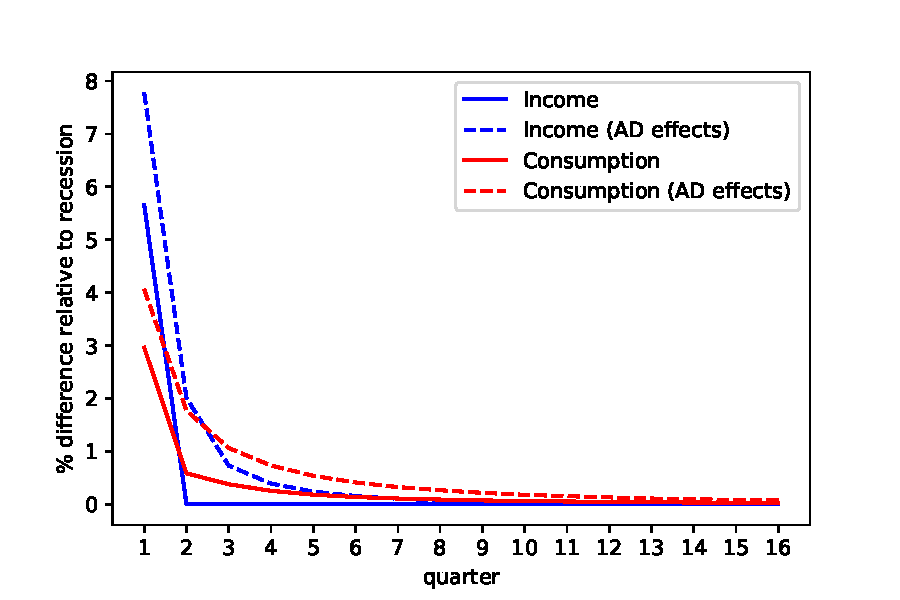
\includegraphics[width=0.8\linewidth]{Code/HA-Models/FromPandemicCode/Figures/recession_Check_relrecession}
	\caption{Impulse responses of aggregate income and consumption to a stimulus check during a recesssion with and without aggregate demand effects}
	\label{fig:recessioncheckrelrecession}
\end{figure}

Figure \ref{fig:recessioncheckrelrecession} shows the impulse response of income and consumption when stimulus checks are issued in the first quarter of a recession. In the model without a multiplier, the stimulus checks account for over 5 percent of the first quarter's income. In the following quarters there are no further stimulus payments and income remains the same as it would have done without the stimulus check policy. Consumption is about 3 percent higher in the first quarter which includes the splurge response to the stimulus check. Consumption then drops to well below one percent above the counterfactual and the remainder of the stimulus check money is then spent over the next few years. In the model with aggregate demand effects, income in the first quarter is almost 8 percent higher than the counterfactual as the extra spending feeds into higher incomes. Consumption in this model jumps to a higher level than without aggregate demand effects and comes down more slowly as the feedback effects from consumption to income dampen the speed with which income---and hence the splurge---return to zero. After a couple of years, when the recession is most likely over and aggregate demand effects are no longer in place, income is close to where it would be without the stimulus check policy although consumption remains somewhat elevated.

\begin{figure}
	\centering
	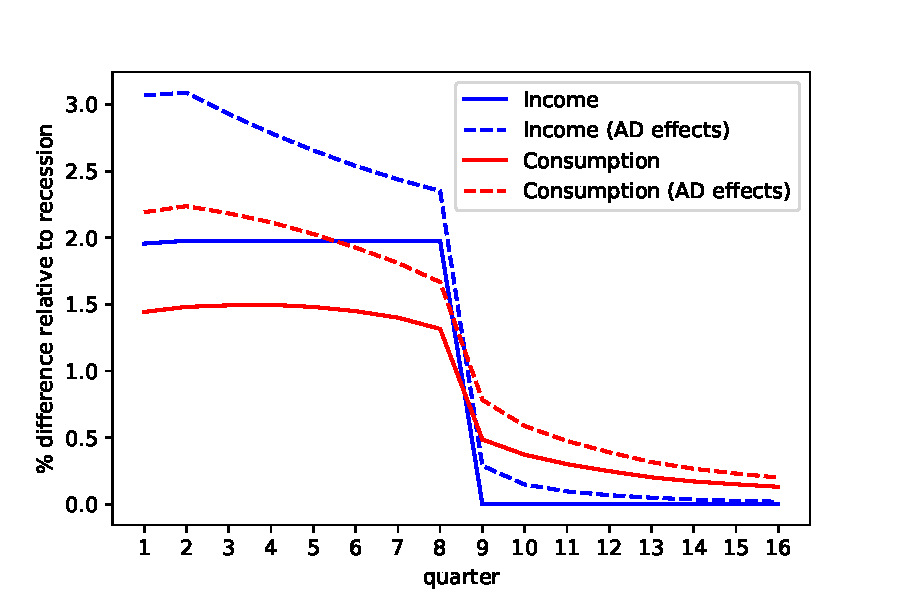
\includegraphics[width=0.8\linewidth]{Code/HA-Models/FromPandemicCode/Figures/recession_taxcut_relrecession}
	\caption{Impulse responses of aggregate income and consumption to a pay roll tax cut during a recesssion lasting eight quarters with and without aggregate demand effects}
	\label{fig:recessiontaxcutrelrecession}
\end{figure}

Figure \ref{fig:recessiontaxcutrelrecession} shows the impulse response for a payroll tax cut that persists for two years (8 quarters). In the model without aggregate demand effects, income rises by two percent as the take-home pay for employed consumers goes up. After the two year period, income drops back to where it would have been without the payroll tax cut. Consumption jumps close to 1.5 percent in response to the tax cut. Over the period in which the tax cut is in effect, consumption rises somewhat as the stock of precautionary savings goes up, before declining in anticipation of the drop in income at the two year mark. Following the drop in income, consumption drops due to the splurge and then decreases over time as consumers spend out the savings they built up over the period the tax cut was in effect. In the model with aggregate demand effect, income rises over three percent above the counterfactual and then declines steadily as the probability the recession remains active, and hence the aggregate demands effects in place, goes down over time.\footnote{Again, consumption tends to first rise due to the build-up of precautionary savings, before falling again as the probability of the recession still in place declines. This hump-shaped pattern feeds through to income, explaining the upward trend in income during the first two quarters.} In response to the now declining expected path for income over the two years during which the tax cut remains in place, consumption also declines, albeit at a slightly slower pace. Following the end of the policy, the savings stock in the model with aggregate demand is high and consumption remains significantly elevated through the period shown.

\begin{figure}
	\centering
	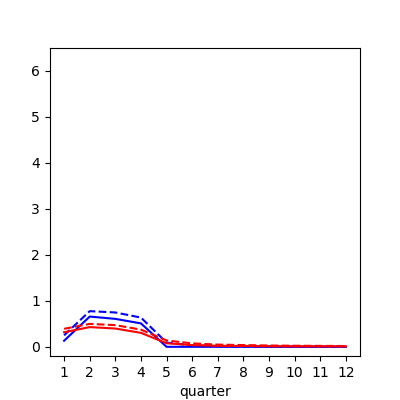
\includegraphics[width=0.8\linewidth]{Code/HA-Models/FromPandemicCode/Figures/recession_UI_relrecession}
	\caption{Impulse responses of aggregate income and consumption to a UI extension during a recesssion with and without aggregate demand effects}
	\label{fig:recessionuirelrecession}
\end{figure}

The final impulse response graph, figure \ref{fig:recessionuirelrecession} shows the response to a policy that extends unemployment benefits from 6 months to 12 months for a period of a year. The path for income, in the model without aggregate demand effects, now depends on the number of consumers who receive the extended unemployment benefits. These consumers are those who have been unemployed for between 6 and 12 months. In the first quarter of the recession the newly unemployed receive unemployment benefits regardless of whether they are extended or not. Therefore, it is in the second and third quarter, when the effects of the recession on long-term unemployment start to materialize, that the extended unemployment insurance payments ramp up. *****QUESTION: why are they zero in the fourth quarter? I thought the policy lasted for one year****** By the fourth quarter, the policy is no longer in effect and income from extended unemployment goes to zero. Consumption in the first quarter jumps up by more than income, prompted both by the increase in expected income and also the reduced need for precautionary saving given the extended insurance. In the model without aggregate demand effects, consumption is only a little above the counterfactual by the time the policy is over. In the model with aggregate demand effect, there is an extra boost to income of about the same size if the first and second quarters. As this extra aggregate-demand induced income goes to employed consumers, more of it is saved and consumption remains elevated several quarters beyond the end of the policy.



\FloatBarrier
\subsection{Multipliers}

In this section we compare the fiscal multipliers across the three stimulus policies. 

Specifically, we employ the cummulative multiplier, which captures the ratio between the net present value (NPV) of stimulated consumption up to horizon $t$ and the full-horizon NPV of the cost of the policy:
\begin{equation*}
M(t) = \frac{NPV(t,\Delta C)}{NPV (\infty,\Delta G)}
\end{equation*}
where $\Delta C$ is the additional aggregate consumption spending up to time $t$ in the policy scenario relative to the baseline and $\Delta G$ is the total government expenditure caused by the policy. The net present value of a variable $X_t$ is given by 
$NPV(t,X) = \sum_{s=0}^{t} \left( \prod_{i=1}^{s} \frac{1}{R_i} \right) X_s$. 

Figure \ref{fig:cummulativemultipliers} plots the cummulative multipliers at different horizons. The stimulus check, which is paid out in quarter one, exhibits the largest multiplier on impact. About 70\% of the total policy expenditure is immediately spent by consumers. After one year and due to the aggregate demand effect, consumption has increased cummulatively by more than the cost of the stimlus check. Over time, the policy reaches a total multiplier of 1.85, see table \ref{tab:Multiplier}.
The multiplier is very similar for the UI extension policy. However, since policy spending here is spread out over four quarters (and peaks in quarter two to three), the mulitplier in the first quarter is considerably lower than in the case of the stimulus check. 
The UI extension policy is very targeted in the sense that it provides additional income to only those consumers, who due to unemployment, have large MPCs. However, some of the spending occurs at later quarters, when the recession might have ended. Overall, around 84\% of the policy expenditure are expected to occur during the recession. In contrast, the check stimulus is paid out fully during the first quarter during which the recession occurs with certainty by construction, such that the AD effect is particularly potent for this policy. Hence while being less targeted and providing stimulus also to agents with low MPCs, the stimulus checks ends up with a relatively high overall mulitiplier due to concentration of spending during the recession.
The paroll tax cut has the lowest multiplier irrespective of the considered horizon. A multiplier of 1 is reached only after around 8 quarters. The total multiplier over the whole simulated period is at approx. 1.3. These relatively small numbers reflect that policy spending lasts long and is thus more likely to occur after the recession has ended. Moreover, only employed consumers with lower MPCs benefit directly from the payroll tax cut. 

Table \ref{tab:Multiplier} contains an additional row (middle) that shows the long-run multiplier for a special case. The aggregate demand effect works through several rounds. First, consumers increase spending due to the stimulus by the policy, which increases income, which in turn boosts consumption. However, this boost in consumption triggers another round of aggregate demand effects, with each round being subsequently smaller in magnitude. In the middle row of the table we show the multipliers that materialize if we only consider the first-round AD effect. (*******Needs more text, why is this interesting to look at?*******)

\begin{table}[h]
	\center
	\input Code/HA-Models/FromPandemicCode/Tables/Multiplier.tex
	\caption{Long-run cummulative multipliers as well as the share of the policy ocurring during the recession}
	\label{tab:Multiplier}
\end{table}

\begin{figure}
	\centering
	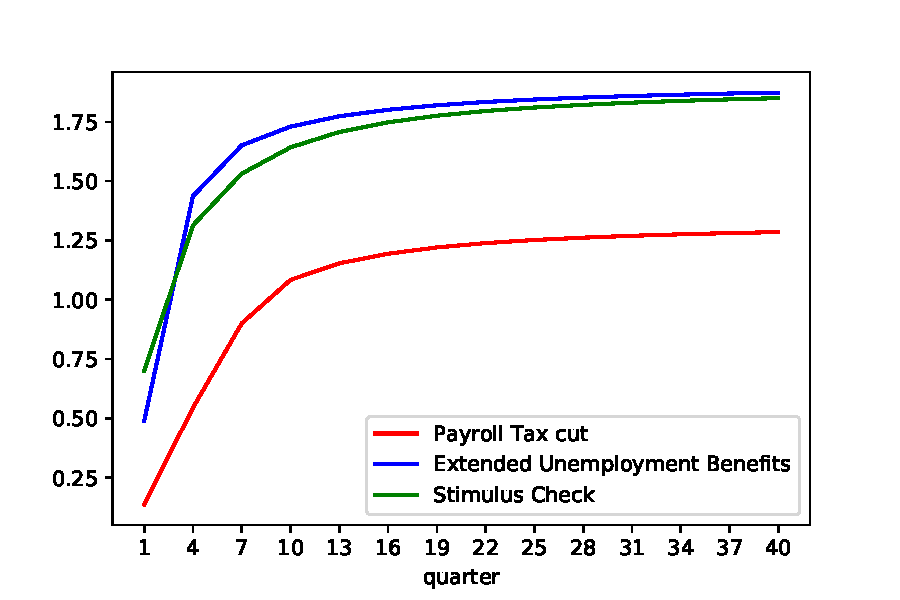
\includegraphics[width=0.8\linewidth]{Code/HA-Models/FromPandemicCode/Figures/Cummulative_multipliers}
	\caption{Cummulative Multiplier as a function of the horizon for the three policies. Policies are implemented during a recession with AD effect active.}
	\label{fig:cummulativemultipliers}
\end{figure}



\end{document}	
